\documentclass[prd, nofootinbib, floatfix, 11pt,tightenlines,times]{article}

\usepackage[paperwidth=8.5in,paperheight=11in,centering,margin=1in]{geometry}
\usepackage{amsmath}
\usepackage{amsbsy}
\usepackage{natbib}
\usepackage{rotating}
\input epsf
\usepackage{amsmath}
\usepackage{wasysym}
\usepackage{subfigure}
\usepackage{graphicx}
\usepackage{epsfig}
\usepackage{color}
%\usepackage{ulem}
%\usepackage{epstopdf}

%\renewcommand{\baselinestretch}{0.98}
\usepackage{epsfig}
\usepackage{titletoc}

\usepackage[toc,page]{appendix}

% HOW TO SET UP AN 8.5 x 11:
% http://www.pages.drexel.edu/~pyo22/students/latexRelated/latexTutorial.html
\topmargin -1.5cm        % read Lamport p.163
\oddsidemargin -0.04cm   % read Lamport p.163
\evensidemargin -0.04cm  % same as oddsidemargin but for left-hand pages
\textwidth 16.59cm
\textheight 21.94cm 
\parskip 7.2pt           % sets spacing between paragraphs
\parindent 0pt		     % sets leading space for paragraphs

%%%%%%%%%%%%%%%%%%%%%%%%%%%%%%%%%%%%%%%%%%%%%%%%%%%%%%%%%%%%%%%%%%%%%%
% set up formatting of python code
%
% to use insert python code, you can use
% \begin{python}
% ...
% \end{python}
\usepackage{listings}
\usepackage{color} % Used for syntax highlighting.
\usepackage{textcomp} % Used for syntax highlighting.

\renewcommand{\lstlistlistingname}{Code Listings}
\renewcommand{\lstlistingname}{Code Listing}
\definecolor{gray}{gray}{0.5}
\definecolor{key}{rgb}{0,0.5,0}
\lstnewenvironment{python}[1][]{
\lstset{
language=python,
basicstyle=\ttfamily\small,
otherkeywords={1, 2, 3, 4, 5, 6, 7, 8 ,9 , 0, -, =, +, [, ], (, ), \{, \}, :, *, !},
keywordstyle=\color{blue},
stringstyle=\color{red},
showstringspaces=false,
emph={class, pass, in, for, while, if, is, elif, else, not, and, or,
def, print, exec, break, continue, return},
emphstyle=\color{black}\bfseries,
emph={[2]True, False, None, self},
emphstyle=[2]\color{key},
emph={[3]from, import, as},
emphstyle=[3]\color{blue},
upquote=true,
morecomment=[s]{"""}{"""},
commentstyle=\color{gray}\slshape,
framexleftmargin=1mm, framextopmargin=1mm, frame=shadowbox,
rulesepcolor=\color{gray},#1
}}{}
%%%%%%%%%%%%%%%%%%%%%%%%%%%%%%%%%%%%%%%%%%%%%%%%%%%%%%%%%%%%%%%%%%%%%%

\definecolor{orange}{rgb}{1.00,0.65,0.00}
\def\arcsec{^{\prime\prime}}

\newcommand{\becker} { \textcolor{orange} {
\ensuremath{\blacksquare} {\bf AndyB:}  
\ensuremath{\blacksquare} } }

\newcommand{\simon} { \textcolor{red} {
\ensuremath{\bigstar} {\bf Simon:}  
\ensuremath{\bigstar} } }

\newcommand{\ajc} { \textcolor{blue} {
\ensuremath{\clubsuit} {\bf AndyC:}  
\ensuremath{\clubsuit} } }

\newcommand{\yusra} { \textcolor{cyan} {
\ensuremath{\diamondsuit} {\bf Yusra:}  
\ensuremath{\diamondsuit} } }

\newcommand{\russ} { \textcolor{green} {
\ensuremath{\natural} {\bf Russell:}  
\ensuremath{\natural} } }

\newcommand{\comment}[1]{{\color{cyan} [{comment: #1}]}}

%\titlecontents{subsection}[4.8em]{}{\contentslabel{2.4em}}{\hspace*{-2.8m}}{...}
%\titlecontents{subsubsection}[6.0em]{}{\contentslabel{2.4em}}{\hspace*{-2.8m}}{}

\author{Andrew Becker, Simon Krughoff, Andrew Connolly, Yusra AlSayyad, Russell Owen}
\title{Roadmap for Winter2013 Production}
\date{\today}

\begin{document}

\maketitle

The goal of late Winter2013 production is the testing of image
subtraction algorithms and the exercise of the {\tt ip\_diffim}
package.  The package will be utilized at 3 distinct portions of the
production pipeline: in the subtraction of Snaps for the rejection of
cosmic rays; in the matching of input images for a Psf--matched
template; and in the subtraction of this template from individual
science Exposures.

The input data will be subsets of the simulated LSST images (ImSim);
stretch goals include application of the algorithms to SDSS Stripe82
data (S82).  The processing steps for the ImSim data include:
application of the Isr pipeline; combining the two Snaps in a Visit
into a single Exposure; calibration, detection, and measurement on the
Exposure; stacking of multiple Exposures into a Psf--matched template
image; subtraction of this template from single--epoch Exposures;
detection, measurement, and characterization of DiaSources that remain
in the difference image; and ingestion of these DiaSources into a
MySQL database.  The natural QA hooks are in the assessment of the
Psf--matched template, and in the purity of the DiaSource sample.  We
will focus on the following metrics to assess the production:
\begin{itemize}
\item rate of false positives (purity)
\item rate of missed known or expected detections (completeness)
\item performance (computational and I/O)
\end{itemize}
This document outlines the details of each stage of production, 
including estimates of compute time and required development tasks.

\clearpage
\tableofcontents
\clearpage

%%%%%%%

\begin{sidewaysfigure}
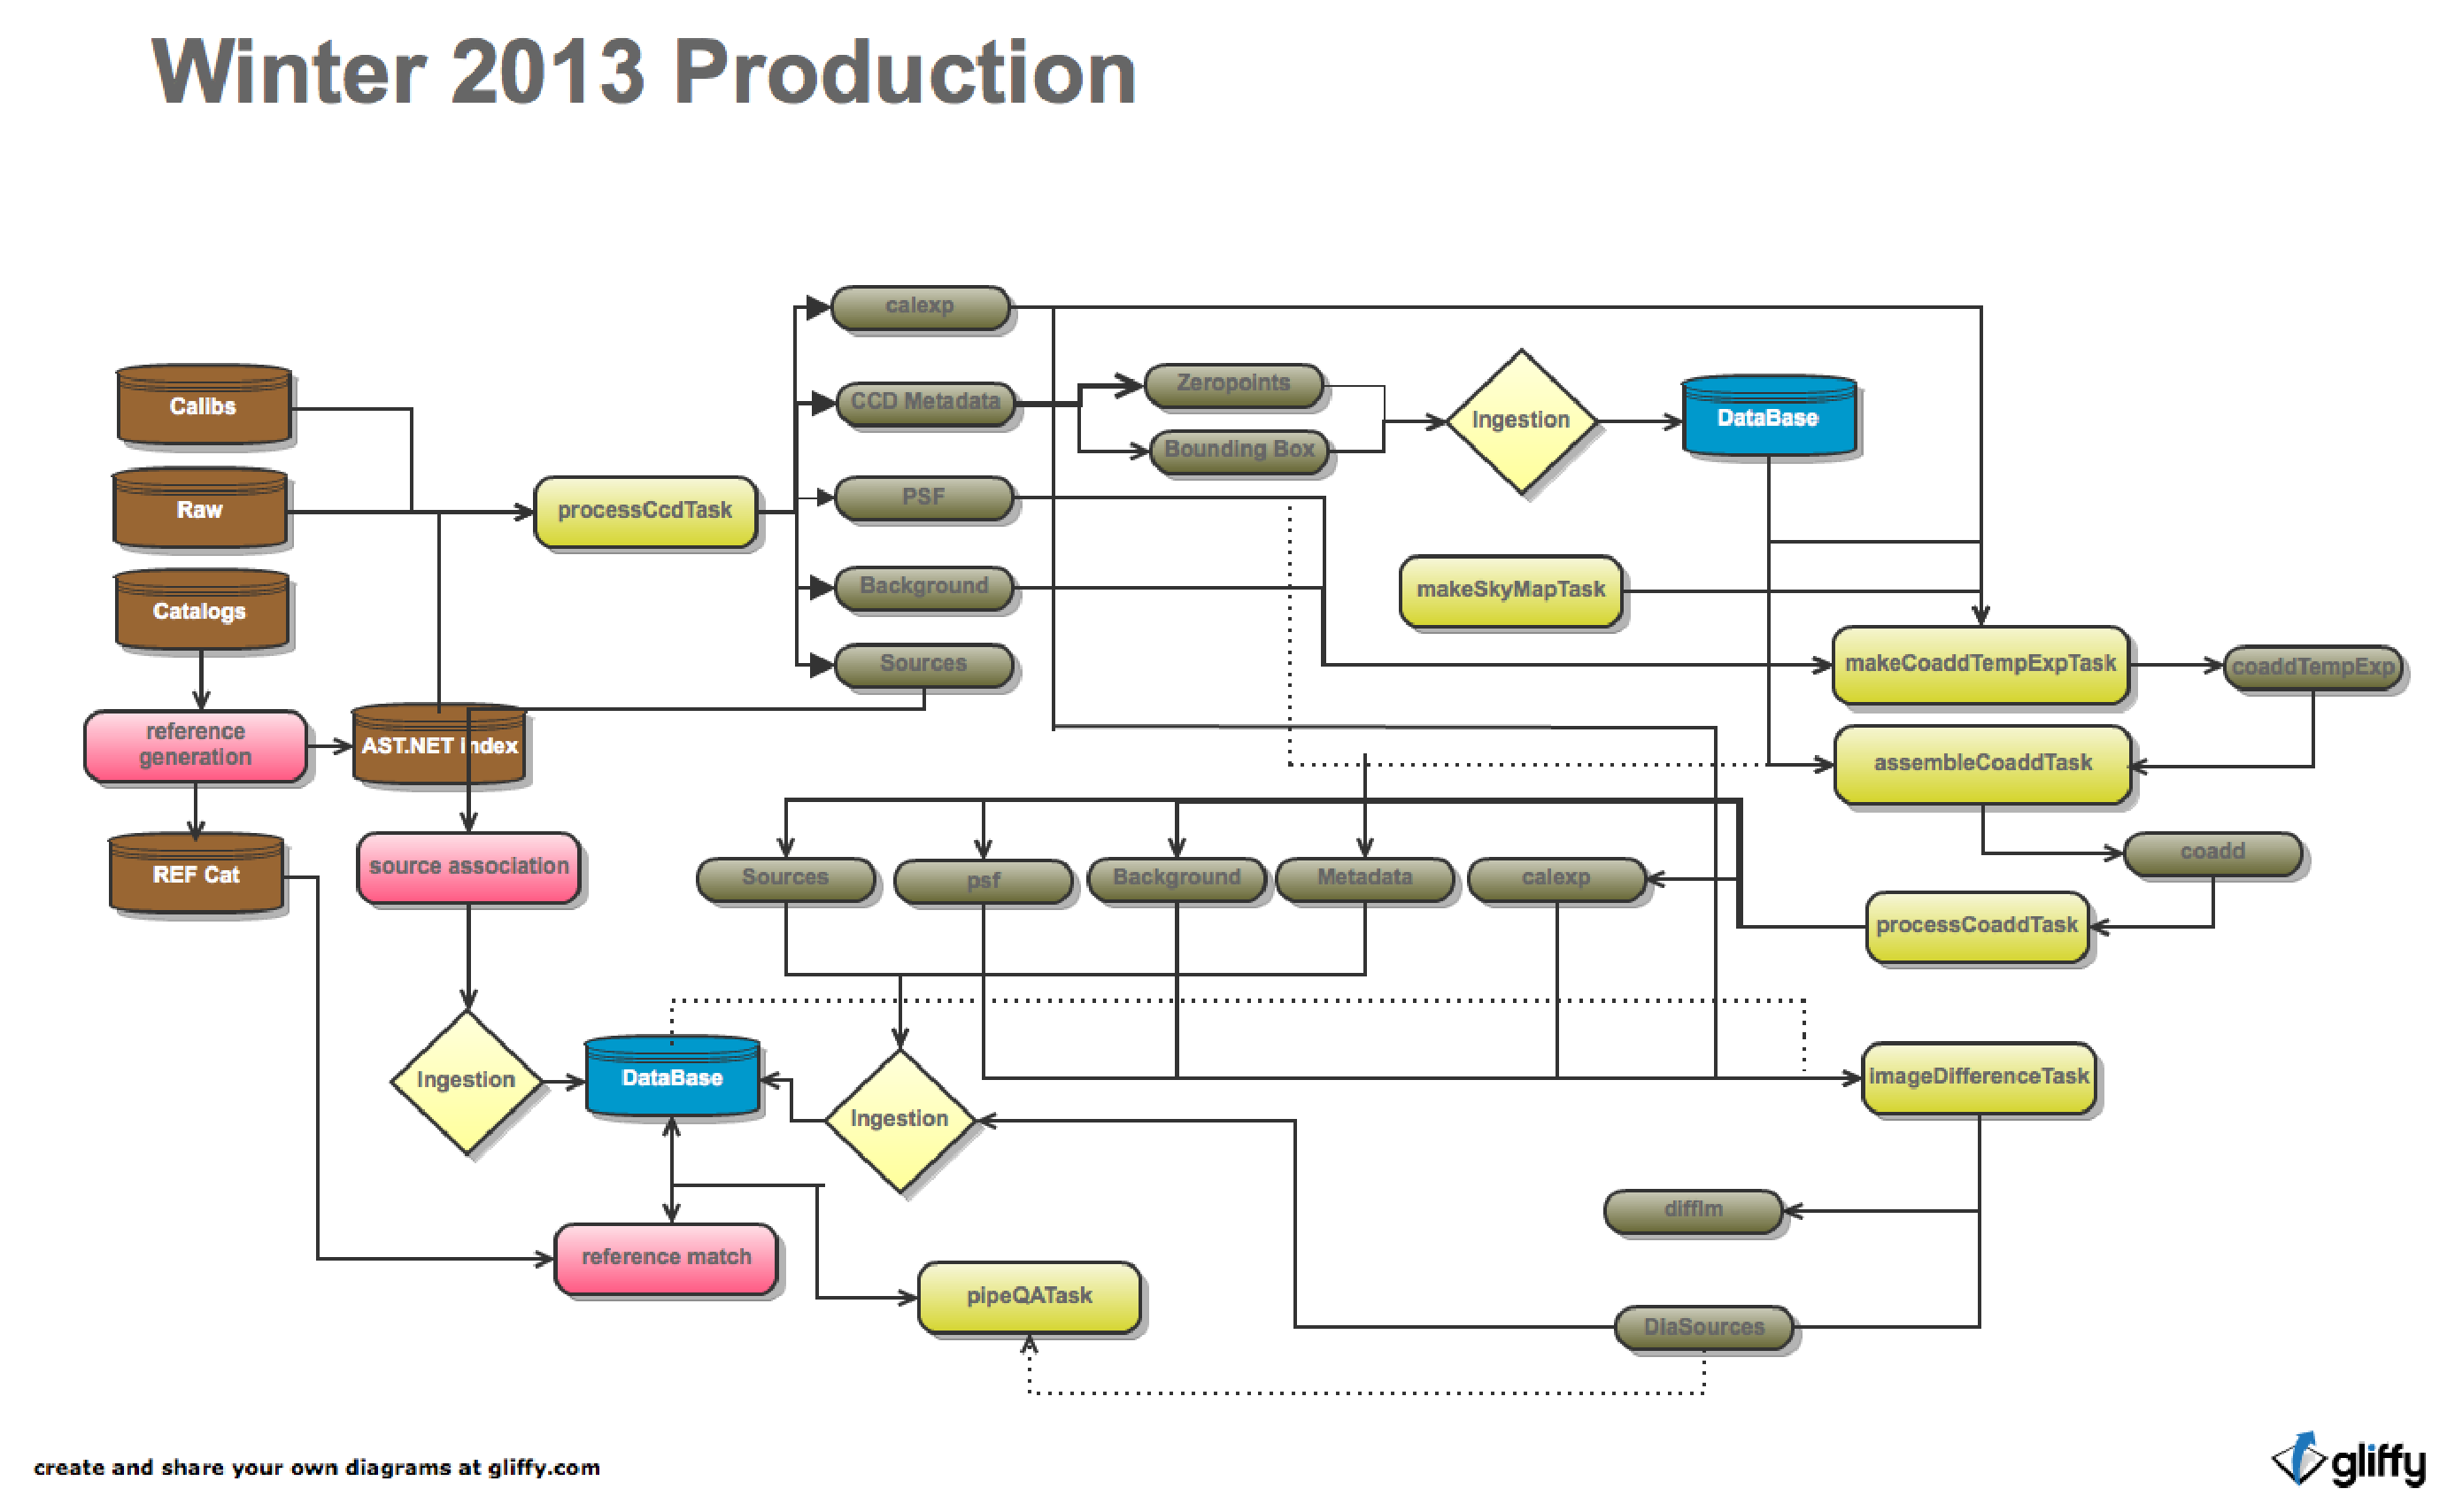
\includegraphics[width=\textwidth]{Figures/Winter_2013.eps}
\caption{Flow of primary information in image differencing. Brown
  boxes are input data, blue boxes represent the database, yellow
  represent ingestion into the database. Grey-brown boxes are derived
  data and yellow-green boxes are the individual pipeline tasks (applications
  that exist but not in the form of pipeline tasks are shown in pink).}
\label{flow}
\end{sidewaysfigure}

\clearpage 

\section{Simulated data} 

Three sets of simulated data are available for use in development of
image differencing: 5yr, Wide, and Deep. These are described in detail
at: \\ {\tt http://dev.lsstcorp.org/trac/wiki/ImSim/Summer2012Plan}.
Development of the LSST algorithms for Winter 2013 (W13) will focus on
subsets of the 5yr data, which comprise 2369 visits (full focal plane)
of 5 adjacent fields observed over a 5-year period in the full suite
of filters. All fields are dithered (spatially and rotationally), with the
spatial dithering defined with a minimum and maximum dither size of
0.2 and 1.75 degrees, respectively. Rotational dithering is based on
{\it rottelpos} (the angle of the camera with respect to the
telescope) as given by OpSim 3.61.

The depth maps derived from the positions of the 5yr data (including
dithers) for the $g$ (176 visits) and $i$ (466 visits) passbands are
shown in Figure~\ref{depth}. All observations are photometric with no
variation in transmission due to clouds. The airmass, sky brightness
and seeing associated with these pointings are given in
Figure~\ref{airmass}. Based on these distributions, the selections on
airmass and time described below all result in data sets of at least
20 visits (equivalent to one year of observations).

\begin{figure}
\centerline{
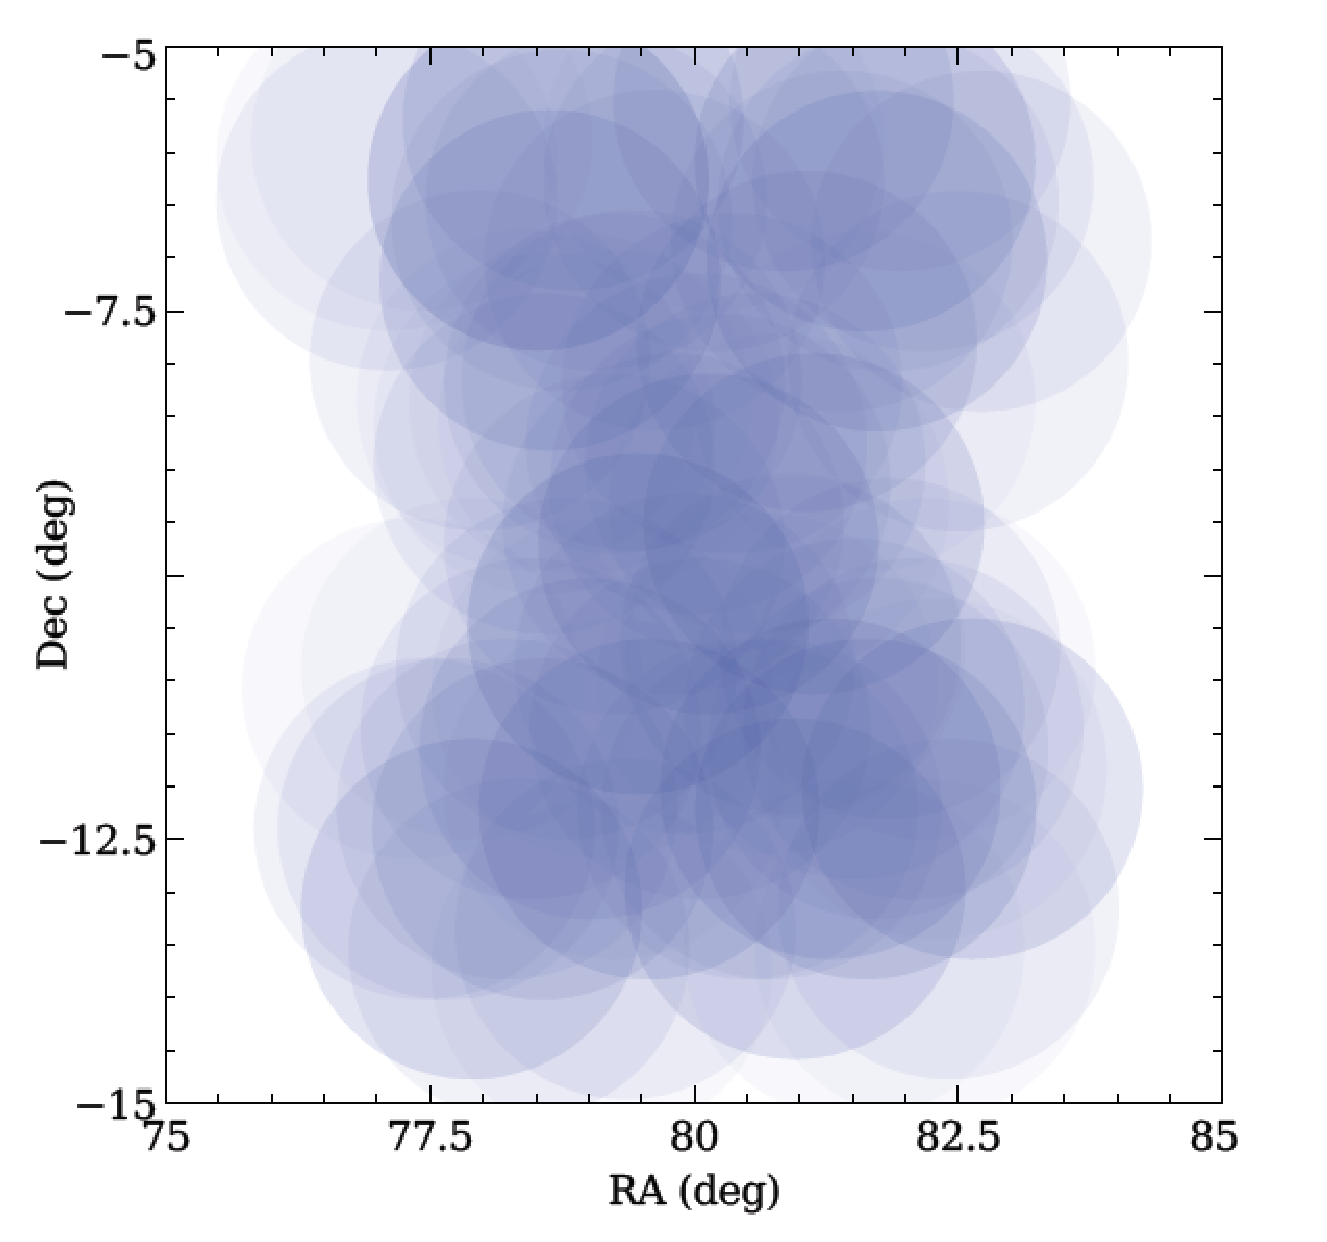
\includegraphics[width=0.4\textwidth]{Figures/depth_g.eps}\hfil
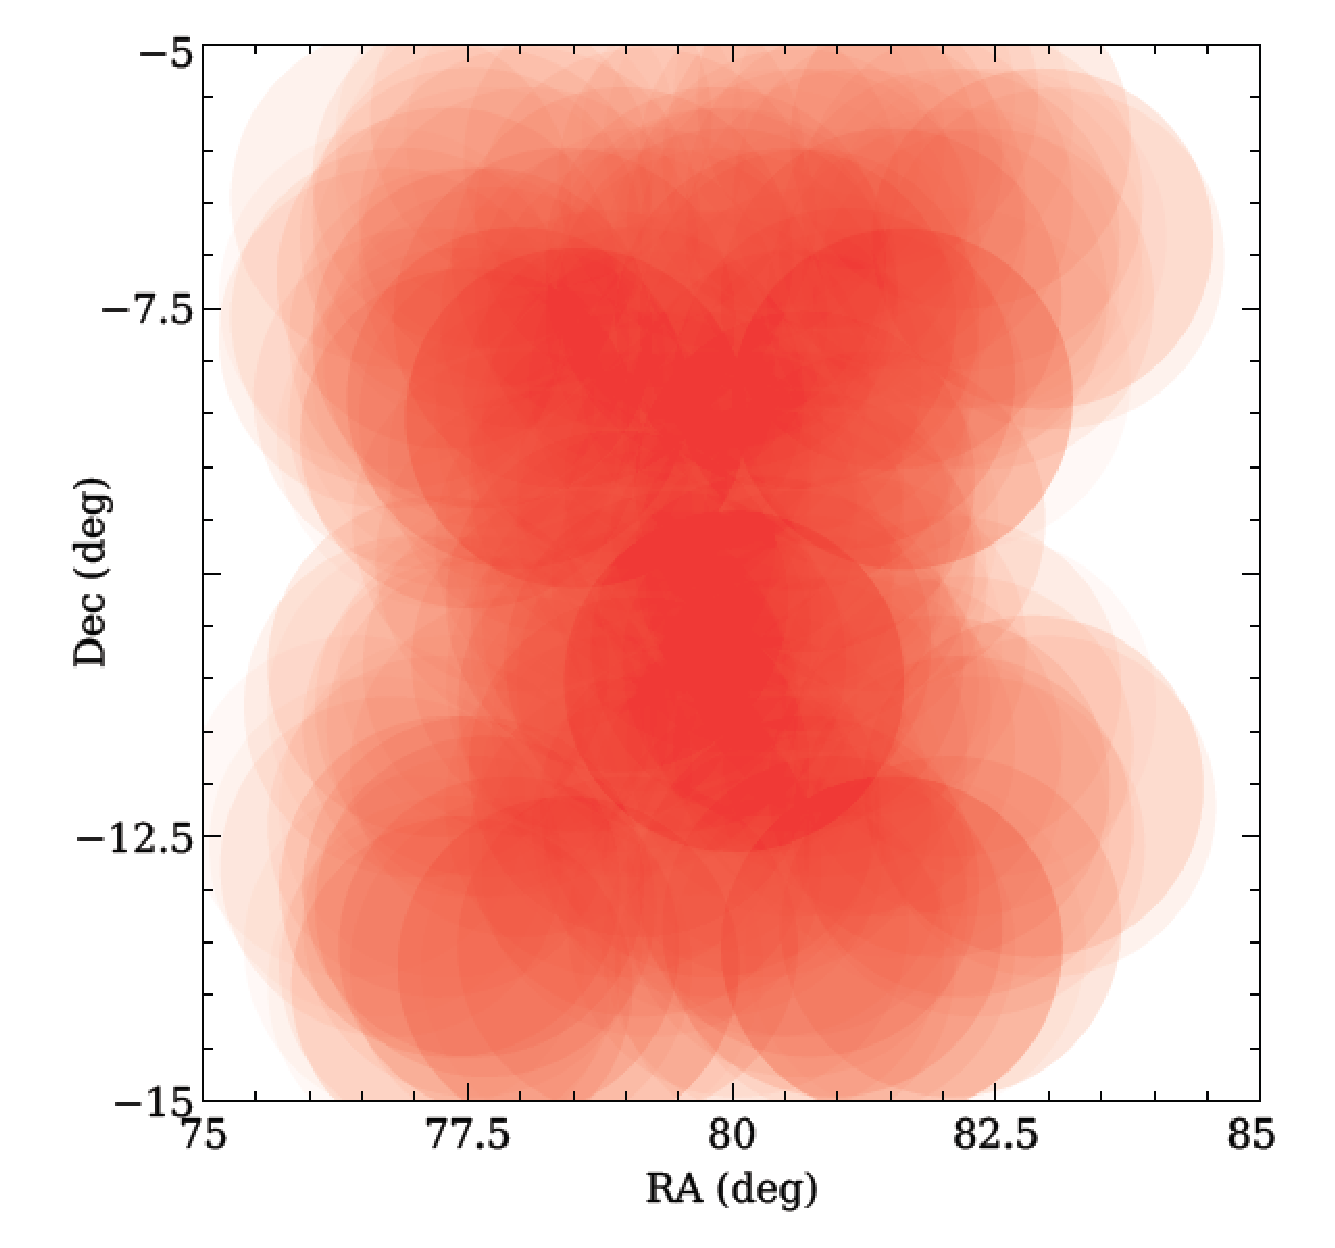
\includegraphics[width=0.4\textwidth]{Figures/depth_i.eps}
}
\caption{The pointing depth map (including dithers) for the 5yr data for the g (left panel)
 and i (right panel)  passbands.}
\label{depth}
\end{figure}


\begin{figure}
\centerline{
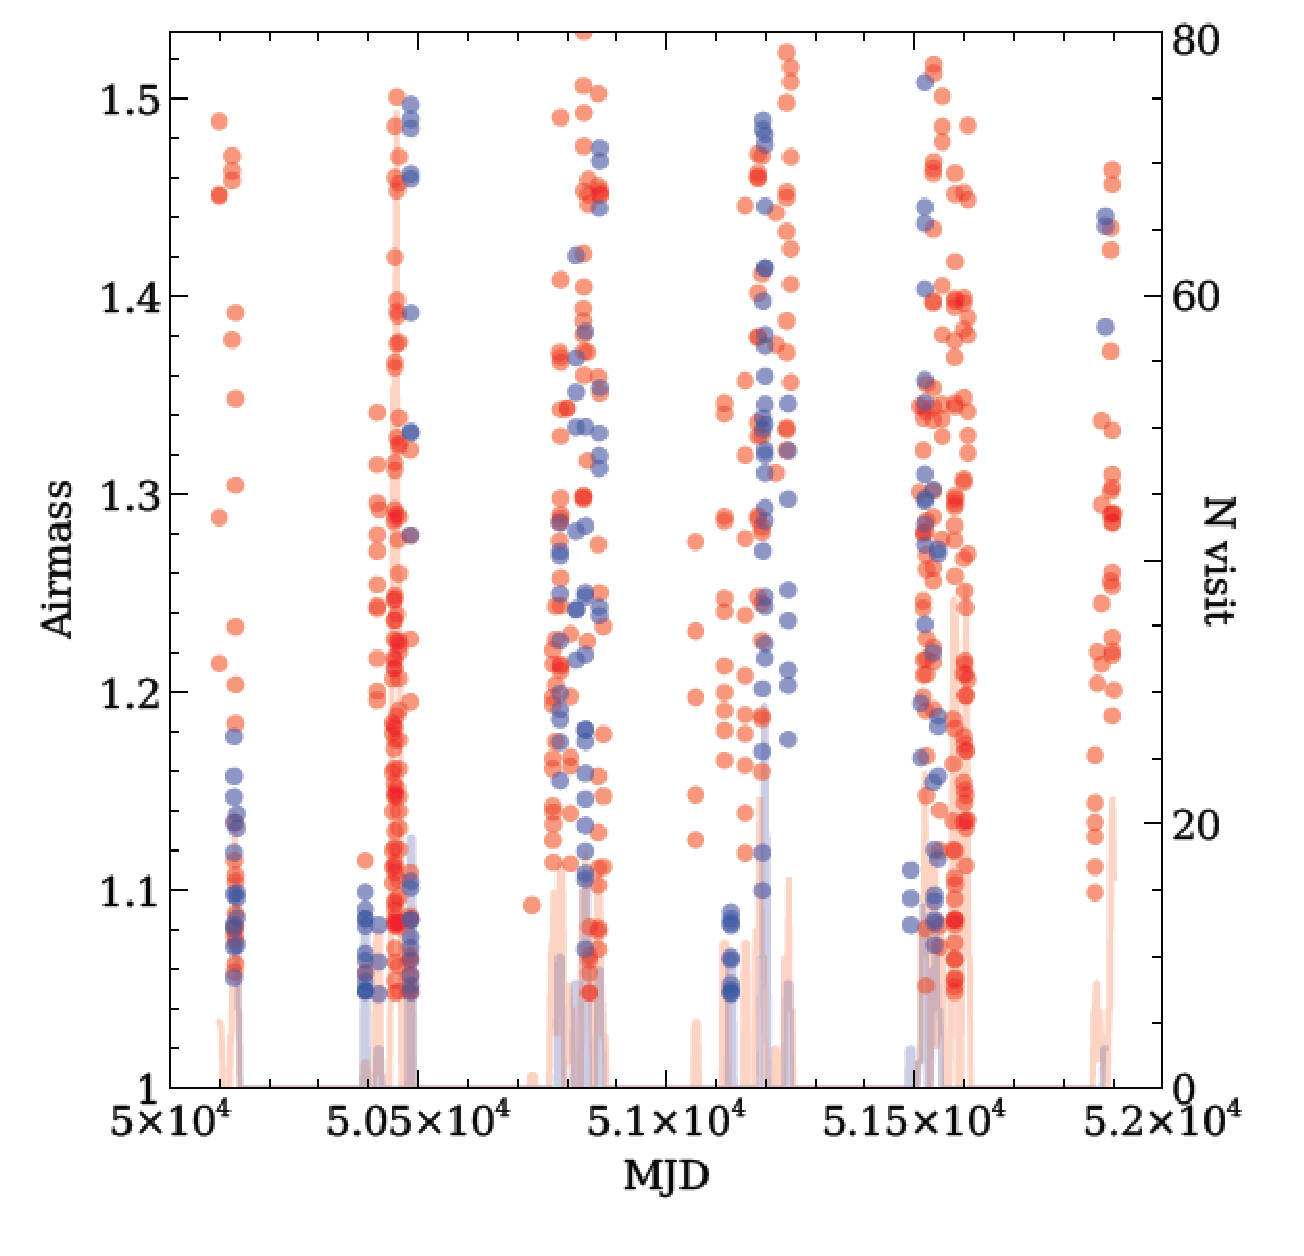
\includegraphics[width=0.3\textwidth]{Figures/airmass_mjd.eps}\hfil
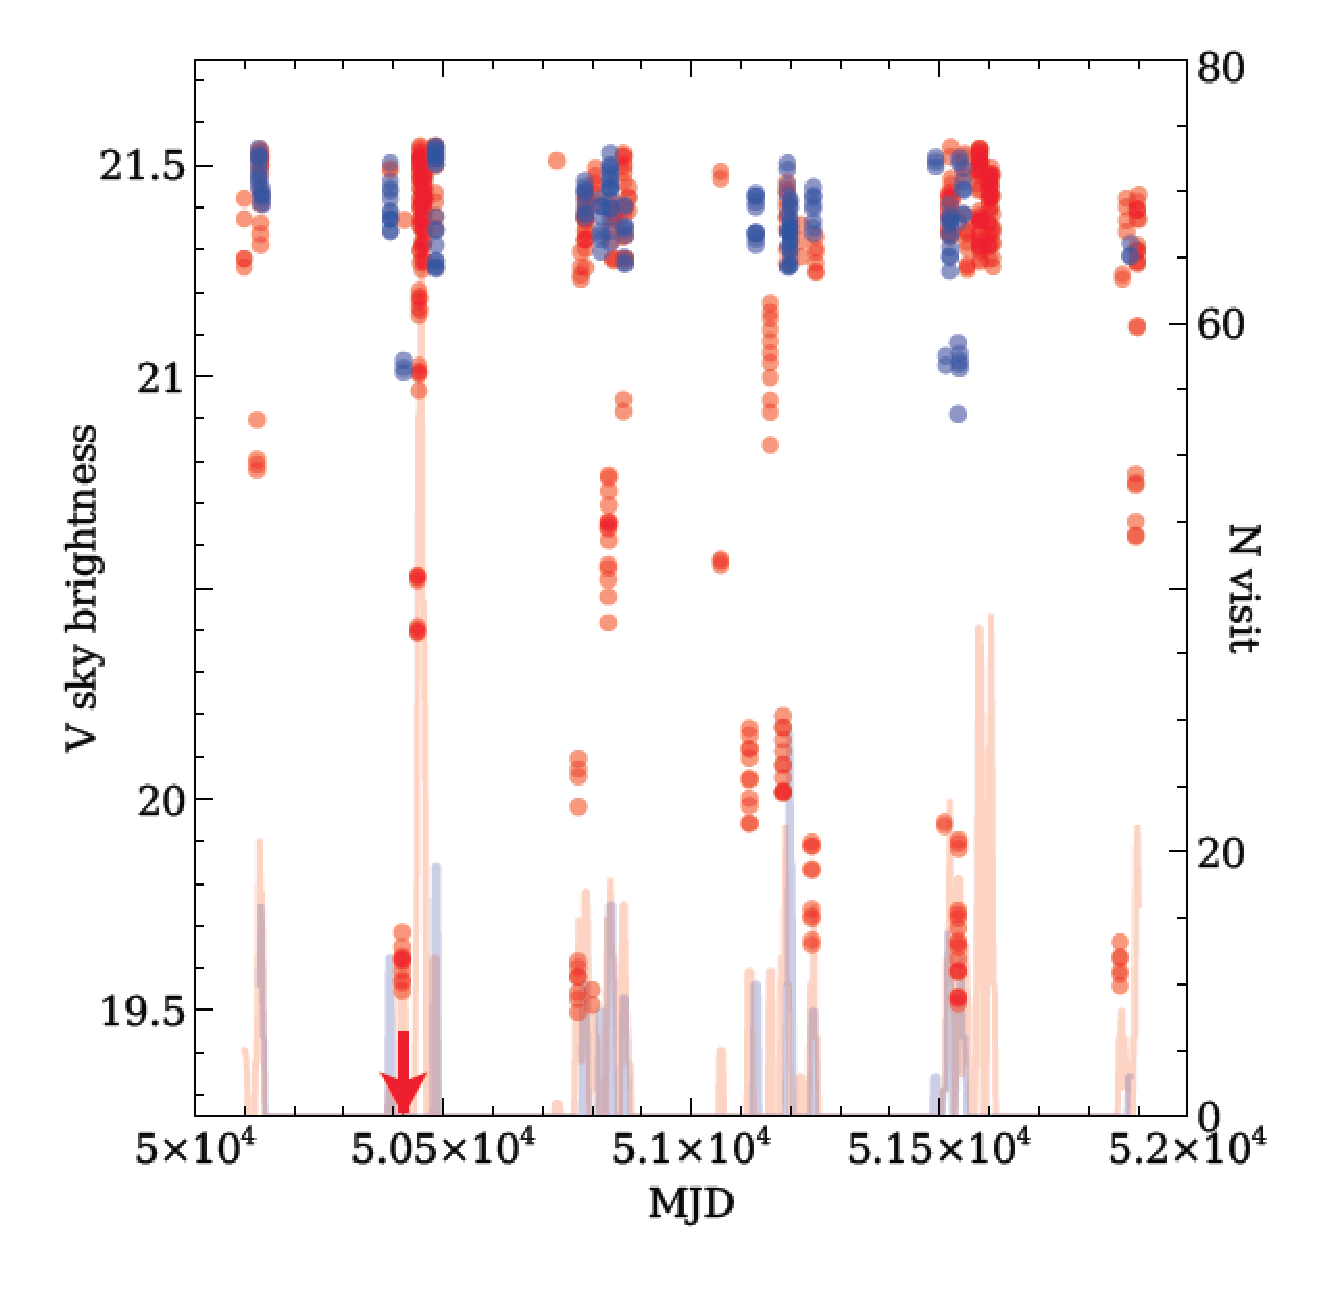
\includegraphics[width=0.3\textwidth]{Figures/sky_mjd.eps}\hfil
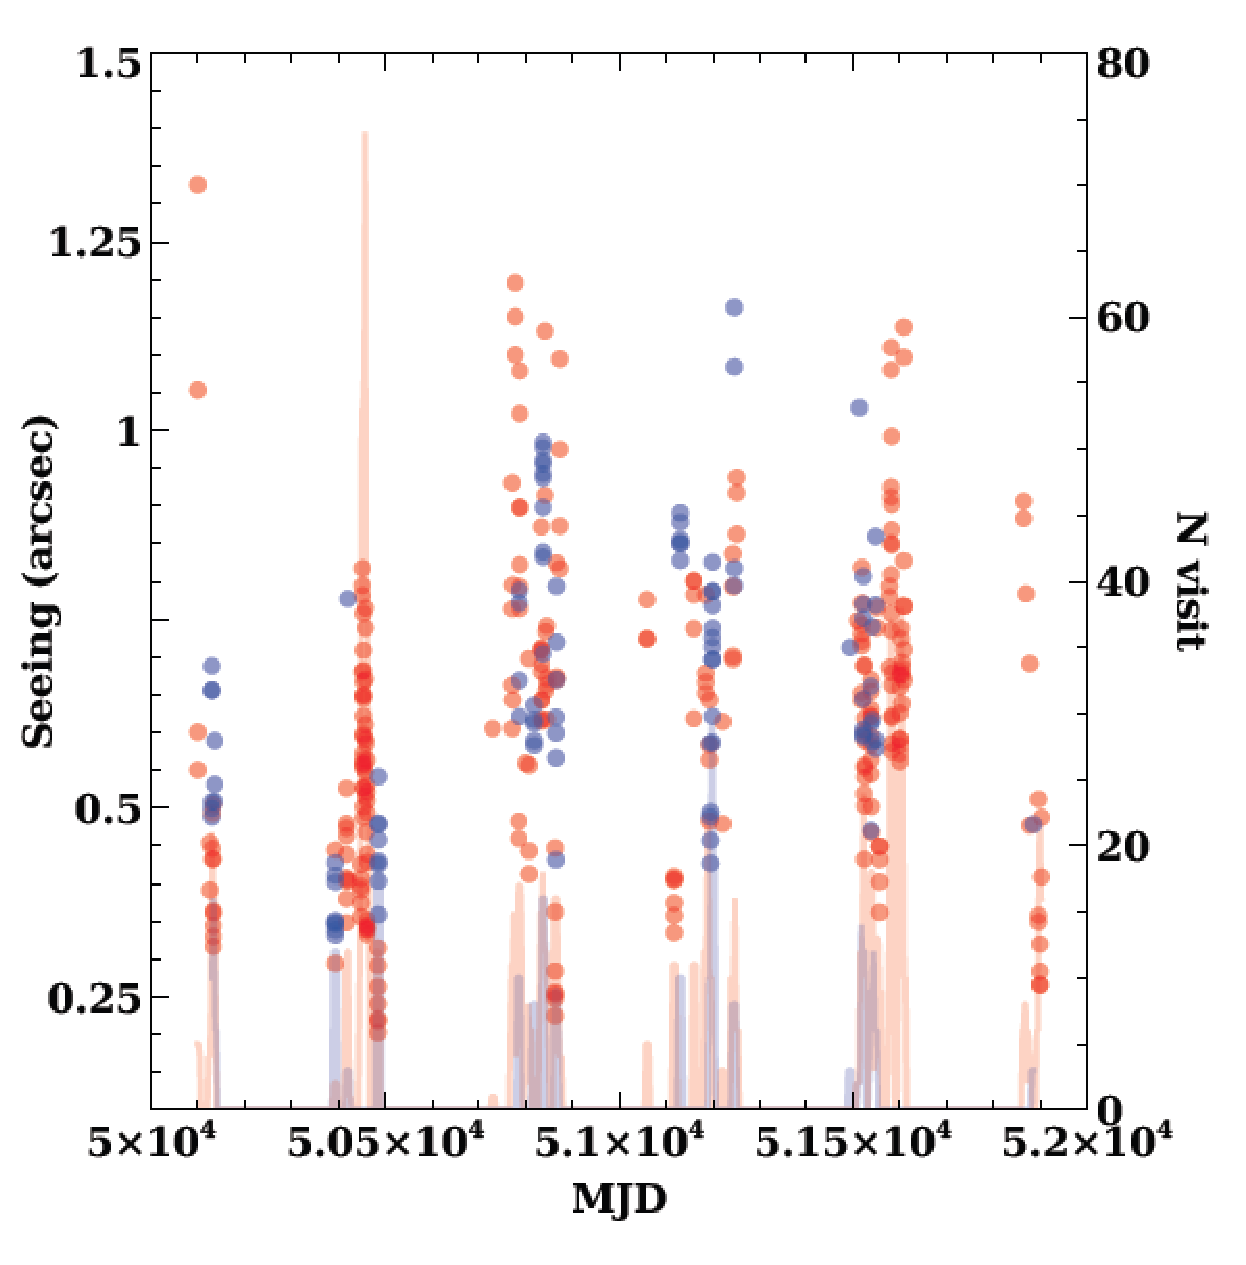
\includegraphics[width=0.3\textwidth]{Figures/seeing.eps}
}
\caption{The airmass, sky brightness, and seeing as a function of MJD for the
  5yr data in the g (blue points) and i (red points) passbands.}
\label{airmass}
\end{figure}

Evaluating the capabilities of the image subtraction software across
the focal plane, and as a function of wavelength (both of the sources
and of the effective filter),  means we must operate on, at a minimum,
full quadrants of the focal plane (as vignetting attenuates the signal
in the outer raft).  In addition, this requires the analysis of observations in multiple
passbands -- one band where chromatic effects are expected to be
negligible ($i$--band) and one where the chromatic effects are
expected to be substantial ($g$--band).

We accomplish this with a series of data sets drawn from the 5yr
simulations. We define a baseline data as the central raft, in the $i$
band, at low airmass, and for a set of observations spread
over 30 days.  This will serve as the reference set that maps out the
performance of the algorithms relative to the optical design of the
LSST and variations in atmospheric seeing. Subsequent subsets of the
simulated data will address the dependence of the image differencing
on position on the focal plane, color, wavelength, time interval
between exposures, differential chromatic refraction, and high proper
motion sources. 
%1% in quadrature at 5 sigma

Figure~\ref{DCR} shows the differential chromatic refraction (DCR) as
a function of airmass (referenced to a G5V star) for a series of stars
ranging from O6 to M8. For main sequence stars in the current
simulated images, we expect the DCR shifts in the $i$ band to be
$<$0.1 pixels for airmass 1.3 and lower and $<$0.05 pixels for
airmasses less than 1.15. The corresponding DCR values for the $g$
band are $<$0.6 pixels and $<$0.4 pixels respectively. Baseline runs
will, therefore, be defined in the $i$--band at airmass $<$1.15.

\begin{figure}
\centerline{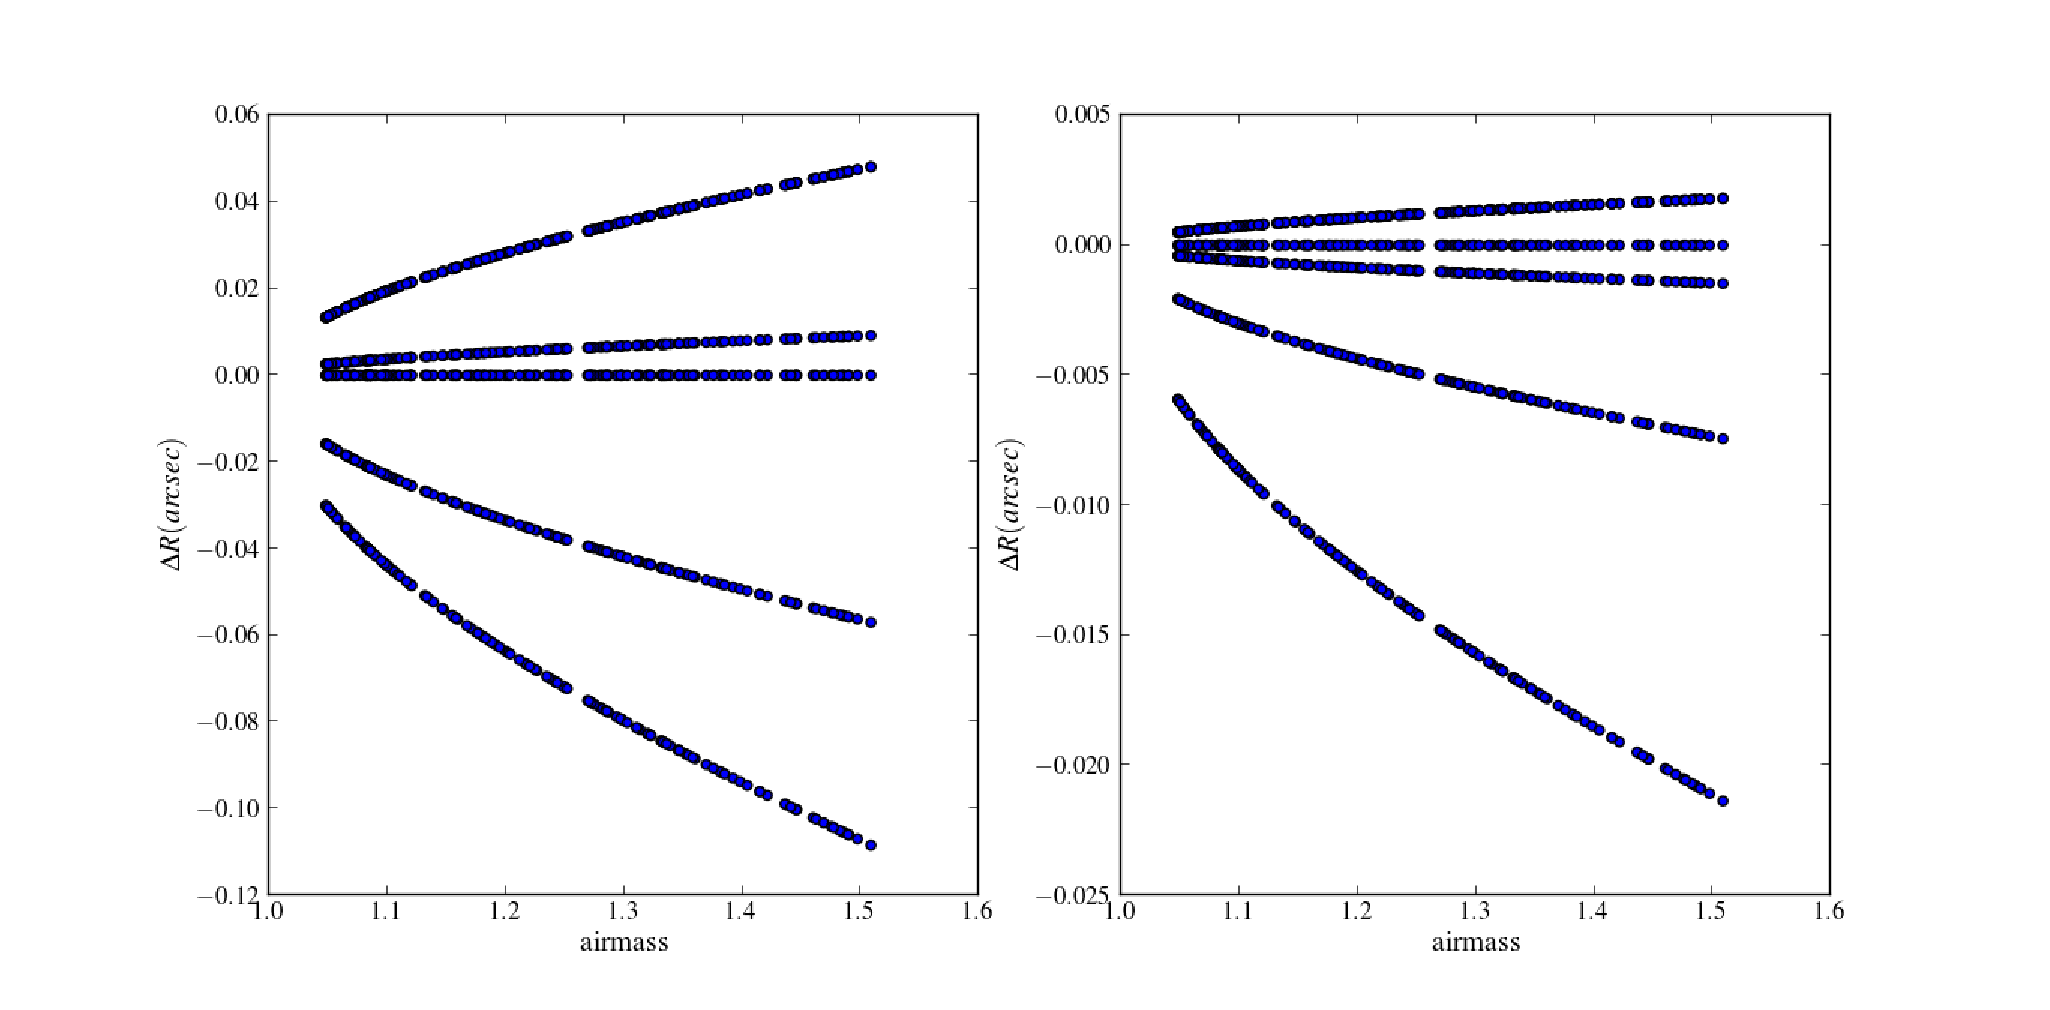
\includegraphics[width=0.8\textwidth]{Figures/DCR_R_stars.eps}}
\caption{The differential chromatic diffraction relative to a G5V star
  as a function of airmass (note different y--scales). The left panel shows the positional offset
  for the $g$ band and the right panel the $i$ band. In both panels
  the stars range in spectral type from main sequence O6 to M8 (top to bottom).}
\label{DCR}
\end{figure}


\begin{table}
\begin{center}
\begin{tabular}{llcrrr}
Sample & Device & Filter & Exposures & airmass & time interval \\
\hline  
Baseline Raft              & central raft  & $i$  & 20 & $<$1.15 &$<$30 days \\
Baseline Focal Plane   & focal plane  &  $i$ & 20 & $<$1.15 &$<$30
days \\
\hline  
Color Raft              & central raft  & $g$  & 20 & $<$1.15 &$<$30 days \\
Color Focal Plane   & focal plane  &  $g$ & 20 & $<$1.15 &$<$30 days \\
\hline 
Time Raft              & central raft  & $i$  & 20 & $<$1.15 &$>$3 years \\
Time Focal Plane   & focal plane  &  $i$ & 20 & $<$1.15 &$>$3 years \\
\hline 
DCR Raft              & central raft  & $g$  & 20 & $>$1.3 &$<$30 days \\
DCR Focal Plane   & focal plane  & $g$  & 20 & $>$1.3 &$<$30 days
\end{tabular}
\end{center}
\end{table}



Master flats, darks, and biases will be produced by coadding 10
examples (each including 2 snaps).  Time dependent effects will not be
simulated in the calibration products other than those arising from
the spider. The spider introduces asymmetric vignetting.  This will be
taken out using flat fields produced with a variety of rotator angles.
Where the effect is strongest (the outermost 4 CCDs), the angular
dependence introduces scatter of $\sim 5$\%.  Using flats generated at
increments of 5 deg from 0 - 90 deg (18 master flats) will bring this
below the nominal 1\% error.


{\bf Reference Catalogs}\\

Reference catalogs for entire W13 5yr survey exist for stellar sources
and will be generated for galaxy sources. The attributes of the
reference catalog will be extended (from S12) to include:

-- unique integer id of the object traceable back to the base catalogs

-- RA position of the object centroid in degrees

-- DEC position of the object centroid in degrees

-- {u,g,r,i,z,y} observed LSST magnitudes (in the mean sense for variable objects)

-- proper motion in RA marcsec/yr

-- proper motion in Dec marcsec/yr

-- object class id (main sequence star, wd, bhb, etc.)

-- variability class (Agn, M-dwarf flare, RRly, etc.  0 if not variable)

-- galaxy position angle in degrees 

-- galaxy semi-major axis 

-- galaxy semi-minor axis

-- bulge to total ratio

-- Agn to total ratio

-- disk to total ratio

-- Agn variability parameters (tau and SF\_{u,g,r,i,z,y})

-- A\_v reddening 

\subsection{Evaluation and Development}

-- Generation of galaxy reference catalogs for the selected W13 fields

-- Creation of astrometry.net index files for the reference catalogs

-- Generation of angle dependent flats (360 visits) and evaluation
that 5 degree sampling produces photometry good to 1\%

-- Generation of visit specific reference catalogs that will capture
the  variability of the sources at the point of observation.

All specified data are currently stored at NCSA.  Special purpose runs
can and will be undertaken as needed using the Google resources and
will be staged at JHU and then transferred to NCSA.  


%\clearpage 
\section{CreateCalibrationProductsTask} 
This task takes individual calibration frames and combines them into
high signal-to-noise (S/N) master frames.  The masterbias, masterdark,
and masterflat will be applied to the input calibration data. This task will
not be camera specific and will be overridden by camera specific
configs (and potentially using the config to retarget subtasks) in the
camera obs package.  The general flow of data will be to process the
individual frames with the appropriate instrument signature removal
(ISR) steps for the product and camera.  Normalization of the flats is
applied relative to the full focal plane. Most of the components of
this task have been implemented using a combination of ImSim specific
code and code written by Paul P. for Subaru.

\subsection{Input/Outputs}
Inputs are: A set of raw calibration frames.

Outputs are: A set of master calibration frames.

\subsection{CalibrationProcessTask subTask}
This is an ISR-like task that corrects the frames for instrumental effects for that calibration
product.

\subsection{CalibrationScaleTask}
This task is responsible for
scaling all flats in a focal plane so that there is a single normalization for the full focal plane.

\subsection{CalibrationCombineTask}
The individual calibration frames are combined into a single high S/N master frame. 

\subsection{Evaluation and Development}

-- Design review to address implementation issues.

-- Implementation of process, scale and combine as pipeline tasks

-- Evaluation of the required sampling of the angular dependent flat
fields in terms of the required photometric accuracy


%%%%%%%

%\clearpage 
\section{ProcessCcdTask\label{processccdsec}} 
The ProcessCcdTask takes input data from its raw form to a calibrated
and photometered science image. The ProcessImageTask task is
subclassed with camera specific configs and processing. The work flow
initially removes the instrument signature, which is handled by the
camera specific subclass.  For ImSim data, individual snap images can
then be combined before the rest of processing happens. Calibration
measures the Psf and aperture correction, and generates the
photometric and astrometric calibration.  In the detection task
footprints are deblended and measurement is run on the deblended
footprints.  Most of the above steps are optional, but care is
required when turning any one off to determine the effects on downstream processing.

\subsection{Input/Outputs}
Inputs are:

-- Two raw science frames (as Snaps)

-- Astrometry.net index files for photometric and astrometric calibration

-- Master calibration frames


Outputs are:

-- Exposure metadata for ingest (bboxes, zeropoints, etc.)

-- Sources for ingest

-- Calexp for input to {\tt ip\_diffim}

-- Background to add to Calexp for {\tt ip\_diffim}

-- Psf for Psf matching

\subsection{IsrTask subTask}
The ISR is handled by a camera specific task in the camera obs
package.  For ImSim the process is overscan subtraction, bias
correction, flat correction, assembly of amps into a chip--sized
image, and interpolation of saturated and bad pixels.

\subsection{SnapCombineTask subTask}
The baseline LSST observing plans defines a field ``visit'' as the
acquisition of two back--to--back images (snaps) and their combination
into a single visit Exposure.  CRs can be detected by subtracting two
snaps (snap2 - snap1). Objects with either positive or negative
polarity, indicate a CR in the second or first snap, respectively.
These pixels are masked and interpolated, and the two snaps coadded
into the final visit Exposure.


\subsection{CalibrateTask subTask} 
Calibration interpolates over cosmic rays (if
SnapCombineTask is not run).  An initial (optional)
background subtraction and detection phase is performed.  Detected
sources are used to calculate the Psf, aperture correction, and
photometric zeropoint, and are fed to the astrometry.net framework for
astrometric calibration.

\subsection{DetectTask subTask}
The detect task does an optional second background estimation taking
into account the original detection mask set by the calibrate task.
It then runs final detection.

\subsection{DeblendTask subTask}
The deblend task searches for peaks within the footprints returned by
the detect task and splits the children out into deblended sources.

\subsection{MeasureTask subTask}
The measure task makes the statistical measurements on each footprint (or peak if deblended).

\subsection{Evaluation and Development}

-- Define appropriate configurations for ImSim (including which config
parameters can be turned on and off).
%-- A primary issue is which steps in processCcd can be turned off.  In
%our experience with Stripe82, we found that the products produced by
%essentially all steps were necessary in later processes.  The one
%possible exception was the DeblendTask.  Aperture corrections
%(CalibrateTask) are needed by forced photometry, zeropoints
%(CalibrateTask) are needed by pipeQA and AssembleCoaddTask, and
%detection planes (DetectTask) are needed by the background matching
%tasks.

{\bf ImSim IsrTask}\\
-- Assemble amps in readout order (serial transfer direction is along the x-axis of the image).

%-- Apply the bad pixel masks prior to saturation detection (requires
%generation of bad pixel masks in amplifier coordinates as opposed to
%CCD coordinates)

%Saturation detection is done before bad pixel masking because we have the pixel masks in Ccd coordinates.
%This meant that some bad pixels were also marked as SAT.  We fix this by changing all SAT+BAD pixels back to just BAD
%-- The flats had per chip normalizations meaning that the zeropoint was not fixed for the focal plane.  This should be
%fixed by the new calibration products task

-- Implement a mechanism for the butler to retrieve the appropriate calibration products given a camera rotator angle.

{\bf SnapCombineTask}\\
-- Evaluate the sensitivity of a simple add/subtract approach for
snapCombine as a function of variation in per visit offsets and
variation in PSF. Current simulations have a distribution of offsets
with $>$70\% less than 0.1 pixels but with a 1\% tail extending to 0.6
pixels.

-- Based on the evaluation of the sensitivity: implement Psf-matched
image differencing.

-- Evaluate the appropriate basis functions for psf-matching
(including sum--of--Gaussian basis sets and delta--function kernels),
the spatial order for the interpolation of the kernels,  the
number of bases, and the kernel dimensions.

-- Develop tools to distinguish cosmic rays from the most significant
Snap DiaSource contaminant, the cores of bright stars.  

-- Establish the metadata to be summed (e.g. exposure time), averaged
(e.g. TAI of exposure), and assumed to be the same (e.g. Wcs).


%The outstanding issue driving the decision to use Psf--matching vs. a straight difference
%is the amount of image motion between Snaps in the W13 ImSim data.
%The amplitude of these shifts in the Winter2013 test data, determined
%through manual source detection and matching, is up to 0.12$\arcsec$
%(0.6 pixels).  This amplitude of shift requires that Psf--matching techniques will be necessary for Winter2013 processing.  

%-- Establish if the default spatial order (0) for this model is sufficient.

%-- Establish if the delta function kernel basis set may be used in this Task.
% The delta--function kernel set is more sensitive
%to noise than, but better able to model
%fractional pixel shifts without significant shape distortions.  The
%zero--order spatial model will help to regularize the overfitting
%problem.
%
%-- Establish a sufficient set of basis shapes for the sum--of--Gaussian basis.
%Given the prior expectation that the matching Kernel will look like a delta function, 
%this basis set will be smaller than the default ImagePsfMatchTask set (31 terms).

%-- Decide between the two bases in the final SnapCombineTask Config.

%-- Establish sufficient dimensions for the Psf--matching kernel, since again
%the power is expected to be localized.

%-- Develop tools to distinguish cosmic rays from the most significant
%contaminant, the cores of bright stars.  

%-- Develop tools to query the known cosmic ray list (locations, shapes and amplitudes), 
%and associate them with DiaSources.

%-- Develop tools to query the known star list, and associate them with DiaSources.
%
%-- Develop cuts on measurement features to distinguish cosmics from
%stellar cores in the Snap DiaSources.

%-- Establish the final metadata for the combined Exposure.  E.g. the
%combined Exposure will have an exposure time equivalent to the sum of
%the two input Snaps (i.e. this will {\it not} be an average image). 

{\bf CalibrateTask}\\
-- Evaluate the size of the background grid for background
determination and the configuration parameters.
%. Determine an optimal background grid size; there are several of these in the config
%  and we must understand what each one does.

-- Determine appropriate  aperture sizes for aperture corrections%; the default is too small.

{\bf DeblendTask}\\
-- Define appropriate deblending config

%-- Establish the deblending radius.
%what is this?

{\bf MeasurementTask}\\
-- Define appropriate measurement config (e.g. galaxy shape measurements)
%-- Specify the galaxy shape parameters that will be measured.

\subsection{Metrics and Testing Tools}

-- CR detection and deblending will be evaluated by cross matching
to known sources (variables and cosmic rays) within the reference
catalog or database.

-- Debug tools to associate catalog sources (and measured attributes)
with processed images will be implemented as required

-- Evaluation of the snap combine will be undertaken using the
cross--match of DiaSources with the cosmic ray list, and with the
known star list.

%statistics package and by comparing MSE, numbers of false detections
%etc in the snap difference image.

%Evaluate the cross--match the list of DiaSources  with the cosmic ray list, and 
%with the known star list.  The measured features of these two samples
%will be compared against each other to find the most distinguishing
%characteristics.  We will calculate the efficiency and purity of this
%sample as metrics to optimize.

%%%%%%%

%\clearpage 
\section{MakeSkyMapTask} 

Creates a "sky map": a sky pixelization for Coadds consisting of a
collection of overlapping "tracts".  Each tract is, essentially, a
very large exposure with its own WCS.  Tracts are subdivided into
rectangular overlapping subregions called "patches".

The sky map we plan to use is DodecaSkyMap. It has 12 tracts arranged
as the faces of a dodecahedron.  An alternative if we decide we want
more smaller tracts is HealpixSkyMap which arranges tracts as pixels
in a HEALPix arrangement.

\subsection{Input/Outputs}
 Inputs are:

--  Input and (optionally) output data repository.

Outputs are:

-- A sky map in the output repository.

-- A repository may have two sky maps: one for "deep" Coadds and one for "goodSeeing" Coadds.

\subsection{Evaluation and Development}

-- Evaluate if the distortions at the edge of tracts for DodecaSkyMap
impacts image differencing (e.g.\ due to variations in pixel size or
requirements on the WCS) by modifying the tract boundaries to
intersect with the ImSim data. 

-- Determine if DodecaSkyMap or HealpixSkyMap is the appropriate sky
map definition for W13

-- For HealpixSkyMap, create healpy as an LSST package (healpy is
self-contained other than needing cfitsio).

-- SkyMap unpersistence has been a bit troublesome due to pickling {\it pex\_config} fields.
When {\it pex\_config} changes sometimes this breaks SkyMap unpersistence. We must fix this eventually.
I don't think it's a high priority, but we could try to fix it in time
for late Winter2013 production.

%DodecaSkyMap has large tracts which have significant distortion at
%the edges.  We don't believe this will be an issue for image
%differencing because the template is warped to match the science
%exposure before subtracting. If it does prove to be a problem we can
%switch to using HealpixSkyMap with smaller tracts.



%The overlap between tracts may be larger than necessary, but the main effect of that
%will be to slightly increase storage requirements of Coadds and slightly increase
%the time required to generate them. We will not see either effect in late Winter2013
%because we are only working with a small region on the sky.

\subsection{Metrics and Testing Tools}

No testing is required.  Skymap examples/plotSkyMap prints out useful
information about a sky map and displays a 3d graph of it.

%%%%%%%

%\clearpage 
\section{MakeCoaddTempExpTask} 

Suitable science images for coaddition will be selected based on Psf
FWHM, sky level, and photometric zeropoint.  These images will then be
Psf--matched to a model Psf and warped to the WCS of the desired Coadd
patch to produce a coadd temp exposure ({\tt coaddTempExp}).  The
model Psf will be a circular double Gaussian function, with variable
{\tt sigma1} reflecting the desired FWHM of the Coadd.  This will be
chosen from the distribution of FWHM of the input data, third quartile
for depth and second quartile for good seeing.

All Ccds from a visit that overlap a particular patch are combined
into one coadd temp exposure, so we will create one {\tt coaddTempExp}
per patch per visit.  These {\tt coaddTempExps} are later assembled
into a Coadd by AssembleCoaddTask.

\subsection{Input/Outputs}

Inputs include science exposures {\tt calexp}), a database providing
quality information about those {\tt calexp}, selection criteria, the
desired Coadd type ("deep" or "goodSeeing"), the skymap for that
Coadd, and model Coadd Psf parameters.

The output is a set of {\tt coaddTempExps} ("deepCoadd\_tempExp" or
"goodSeeingCoadd\_tempExp").

\subsection{SelectImagesTask subTask} 

This subTask selects science exposures that are suitable for the Coadd
based on criteria such as Psf FWHM and sky background. It operates by
querying the Science\_Ccd\_Exposure table.

\subsection{ScaleZeroPointTask} 

This subTask photometrically calibrates each {\tt coaddTempExp} to a
common zero point.  In the coadd process, it is important that the
background matcher not try to fit discontinuous offsets in the
background levels. For this reason, the multiplicative scale factor
applied to the {\tt coaddTempExp} should vary smoothly across the
patch. For stripe-82 early production we assumed that the zero-point
in the runs varied smoothly in the R.A direction only.  This will be
expanded to a full two--dimensional model in W13.  The zeropoints are
already calculated in {\tt processCcd} and stored in the
Science\_Ccd\_Exposure table. {\tt ScaleZeroPointTask} pins the
zeropoint down in the center of each Ccd and interpolates a
multiplicative scale factor across the patch.

\subsection{WarpAndPsfMatchTask subTask} 

This subTask first undertakes the Psf--matching of the input {\tt
  calexp} Psf to that desired for the Coadd.  It then astrometrically
warps this Psf--matched image to the astrometric footprint of the
Coadd.  This differs from ImagePsfMatchTask, described in detail in
Section~\ref{sec-imagedifftask}, in one major detail.  In this case,
the {\tt calexp's} {\it model} Psf is read through the butler, and
compared to the idealized Psf that we wish to realize for the Coadd.
Each Psf is realized in a grid of $x,y$ positions to account for
spatial variation of the Psfs.  The two Psfs will be entered into a
KernelCandidate as Images, which it itself entered into a
SpatialCellSet, and sent along to the fitting code where the
functionality is again the same as ImagePsfMatchTask.  Because the
concept of ``variance'' is ill--defined when comparing
model--to--model, all sigma clipping is turned off and the variance is
assumed to have a constant weight.


\subsection{Evaluation and Development}

-- Develop a tool that measures how well Psf matching to a model Psf
works. This likely requires running Psf modeling on a {\tt
  coaddTempExp}.

-- Improve the current Science\_Ccd\_Exposure table and SelectImagesTask.
The only measure of image quality that Science\_Ccd\_Exposure contains is Psf FWHM.
We would like additional information such as Psf ellipticity, airmass and sky brightness.

-- Develop an equation that computes a single measure of quality
based on these various bits of information.



{\bf ScaleZeroPointTask}

-- Fit a 2-D spline to the zeropoints calculated for each Ccd in {\tt
  processCcd}.  {\tt afw} already contains 2-D spline capabilities,
however the only interface at the moment is the {\tt background}
class. The API to the background class only accepts an image. We need
to extend this to be able to accept a list of grid points.

-- Interpolate the scale factor across the patch using the zeropoint
of each star. This is an appropriate application for a Gaussian
Process/Kriging function.

{\bf WarpAndPsfMatchTask}

-- There is trade--off in this process that we will explore in detail.
To illustrate this, we define the dimensions of the {\tt calexp} Psf
as $P \times P$, the FWHM of the Coadd Psf as $C$, and the dimensions
of the Psf--matching kernel as $K \times K$.  When fitting for the
matching Kernel, each Psf image gets convolved with each Kernel basis
function, trimming $K//2$ pixels off of each side due to EDGE effects.
Thus the final number of pixels we have to constrain the Kernel
coefficients are $(P-K) \times (P-K)$.  This means that as the Kernel
gets larger, the number of pixels we have to constrain the solution
gets smaller, and the solution may become unstable.  Providing tension
in the other direction is that if the kernel dimensions are too small
compared to $C$, the kernel stamp may not be large enough to capture
all the power needed to match to that large of a FWHM.  This ends up
yielding ``boxy'' stars in the Psf--matched images.  Ultimately, we
are limited by the dimensions of the {\tt calexp} Psf model $P$, which
in turn sets the maximum size of the kernel such that $(P-K) \times
(P-K)$ provides sufficient ability to constrain all of the Kernel
basis coefficients, which in turn sets the size of the Psf $C$ we may
match to without sufficiently impacting the shapes of the stars, which
in turn sets the number of images that we may include in the Coadd
without deconvolving.  This trade--off, including the definitions of
``sufficient'' above, will be explored in thorough detail in W13
pre--production.

%-- If the model--to--model Psf--matching kernel is too big, we have
%too few pixels to constrain the solution.

%-- If the model--to--model Psf--matching kernel is too small, it
%limits the FWHM of the desired Psf of our coadd (otherwise the stars
%become boxy on the scale of the kernel).

%-- If there is a limitation on the FWHM of the coadd Psf, we are
%limited in the number of images we may use with (FWHM$_i$ $<$
%FWHM$_{Coadd}$), impacting our final depth.

%-- If we wish to increase our depth and include images in the coadd
%with (FWHM$_i$ $>$ FWHM$_{Coadd}$), we will have to deconvolve.

-- Understand ``how much'' deconvolution the code can handle, both in
terms of the fraction of images that were deconvolved, and the degree
to which each of the images is deconvolved, using the measured depth,
variance, and Psf in the Coadd.

-- Establish the quartiles of the FWHM distribution to use for setting
the Coadd Psf, and for including in the Coadd.

-- Establish the impact of {\it not} having color--dependent Psfs (or
Psf--matching kernels) on the Coadd.

-- Science images are presently Psf--matched to a model that is
constant in pixel space.  However, we want to match to a model Psf
that is constant on the sky.  The distortion near the edge of the
LSST's field of view may be large enough that this distinction will
prove significant. Jim Bosch is working on code that will eliminate
this issue by allowing us to warp model Psfs.  However, it is likely
that we will produce some preliminary data before this new code is
ready.

-- Understand the impact of the {\tt meas\_mosaic} package, which is a
port of HSC's \"{u}ber cal, and is necessary to correct known
deficiencies in LSST's {\tt meas\_astrom} package.  This has proven
necessary for creation of non--smeared coadded images, reducing the
RMS of the astrometric fit by a factor of two.

-- Implement minimal spreading of Mask bits in afwMath::convolve.

%We will need to test the following Psf--matching configs:
%
%-- Psf size (set in processCcd)
%
%-- Psf grid 
%
%-- Psf model functions
%
%-- kernel size
%
%We will need to tune our image selection criteria (possibly including our image quality metric)
%to select suitable images.

\subsection{Metrics and Testing Tools}

-- Develop tools to measure the Psf of the {\tt coaddTempExp}.

-- Establish the stability of the model--to--model Psf--matching
kernel as a function of Psf dimension and Kernel dimension by tracking
the condition number of the solution.

-- Evaluate the image quality metric developed for SelectImagesTask.

%%%%%%%

%\clearpage 
\section{AssembleCoaddTask} 

The coadded template image will be constructed using background
matching, as opposed to background subtraction. The assembleCoadd task
assembles a Coadd from a set of {\tt coaddTempExps}.  Each {\tt
  coaddTempExp} is the size of a patch defined by the {\tt skyMap} and
contains pixels from only a single visit.  The {\tt coaddTempExps}
have already been scaled to a common zeropoint and psf-matched.
However, they still have their backgrounds and therefore require
background-matching to a reference visit. The reference visit is
selected based primarily on fractional coverage of the patch and low
background levels and background variance.

The assembleCoadd task assumes that all {\tt coaddTempExps} cannot fit
in memory at the same time. The following steps outline the processing
in more detail:

-- Read in {\tt coaddTempExps} one at a time and fill a list of
weights (inverse mean variance) for each image

-- Pass to the background matching task a list of dataRefIds of the
{\tt coaddTempExp}s, and the reference exposure dataRefId (if
supplied).  Receive back a list of structs containing {\tt Background}
objects and statistics describing the quality of the match.  Prune
this list of exposures, removing the {\tt coaddTempExps} for which the
background-matching failed.  Current tests include too many nans, and
the ratio matchedMSE/diffImVar (defined below).

-- Grid the patch into a smaller sub-region {\tt subBBox}es. For each
{\tt subBBox}, read in each image and keep in memory only the region
that overlaps the {\tt subBBox}. Add the corresponding region from the
Background match to bring the background level up to that of the
reference image.  Coadd by calculating the mean with outlier
rejection.  Repeat for {\tt next subBBox}.  Persist Coadd.

%The image subtraction
%code will also be run using its own internal background--matching (of
%template to science image) model, yielding a difference image with a
%background level of 0.  Currently using a Chebyshev with order 3.

%We need to make sure all necessary metadata ends up in the database.
%This includes zeropoints, sky background, Psf FWHM.

\subsection{Input/Outputs}

Inputs: A repository containing {\tt coaddTempExps} and a skyMap

Outputs: Coadds

\subsection{BackgroundMatchingTask subTask} 
The matchBackground task matches the background of each {\tt
  coaddTempExp} to the level of the reference exposure.  This is done
by fitting a spatial model to the difference of each input exposure
and the reference exposure -- with detections and bad pixels masked
out.  This will equalize the background levels from visit to visit,
while preserving diffuse astrophysical structures.  The task assumes
that all the input {\tt coaddTempExp} are the same size, have been
warped and have been flux-scaled.

Subtract the exposure from the reference exposure, and then pass
generate an afwMath.Background object of this difference image. It
assumes (but does not require or check) that the mask plane already
has detections set; these pixels are ignored.  The 'background' of the
difference image is a collection of grid points that represent the
mean or median difference between images.  These values are smoothed
by spline interpolation (by the Background class), or by polynomial
interpolation by the Approximate class, to yield the background
matching model.

Inputs: 

-- A list of dataRefIds pointing to {\tt coaddTempExps} and an
optional dataRefId to the reference exposure.

Outputs:  

-- backgroundModel: an afw.math.Approximate or an afw.math.Background (Or {\tt None} if fit failed) 

-- fitRMS: RMS of the fit, sqrt(mean(residuals**2))

-- matchedMSE: the MSE of the reference and matched images, mean((refImage - matchedSciImage)**2); 
   this value should be comparable to the mean variance of the difference image.

-- diffImVar: the mean variance of the difference image.

\subsection{Evaluation and Development}

-- Determine the optimal background matching style (polynomial,
spline) and parameters (order, bin size) for the 4000$\times$4000
patches. Differences between Stripe82 data and ImSim data (e.g. the
chip gaps and offsets between Ccds) prevent us from simply reusing the
parameters from early production.

-- Move flux-scaling procedure to {\tt makeCoaddTempExp.py}.
Currently, the assembleCoadd performs the flux-scaling step. This
design was a temporary solution to an early-production problem.  It
would be much more efficient and clean for the flux scaling to be
performed in makeCoaddTempExp.

-- Move the background-matching quality cut to the {\tt
  matchBackgrounds} subtask.

-- Check that API of background matching task is appropriate for {\tt
  ImageDifferenceTask} to match the science image to the template
before subtracting.

-- Determine an appropriate level of sigma clipping to remove known
transients from the Coadd.

-- Write a task that will select a reference run based on the database
that optimizes continuity over a large region of the sky.  By large
region, we mean $>>$ patch.

-- Implement an ``iterative'' Coadd creation process that proceeds by
creating a Coadd using the process outlined above, performing
background subtraction on this Coadd, and using this
background--subtracted Coadd as a reference for background matching
and image subtraction.

\subsection{Metrics and Testing Tools}

-- To test the quality of fit in the background matching step, {\tt
  matchBackgrounds} contains a debugging method that plots the
residuals of the fit.

-- Use the statistics returned for each fit (MSE and variance of the
difference image) to provide an assessment of the interpolation
styles/parameters in development, and to determine if the matching has
been successful in production.

-- Use the Coadd Psf shape, noise properties, and photometric depth to
determine the impacts of deconvolution.

-- Examine the shapes of extreme--color stars in the Coadd to
understand the effects of DCR.


%%%%%%%

%\clearpage 
\section{ProcessCoaddTask} 
We will be running calibration, detection and measurement on Coadds to
generate the data products necessary for QA.  With the outputs of the
ProcessCoaddTask we will answer questions including:

-- Does the measured shape of the Psf match the input model Psf that
the template was designed to have?

-- Does astrometry of the template match the SkyMap?

-- How does the Psf change with position, source flux, etc.?

\subsection{Inputs/Outputs}

Inputs: \\
-- Coadd exposure

Outputs:\\
-- Coadd calexp

-- Coadd exposure metadata

-- Coadd Background model

-- Coadd Psf model

-- Coadd Source catalog

\subsection{Calibrate/Detect/Measure subTasks}
These are identical to those mentioned in \S \ref{processccdsec}.

\subsection{Evaluation and Development}

-- There is no notion of persisting models for QA purposes alone.  For example we will want to persist
the WCS we measure, but only for comparing to the skymap WCS.  In other words, we do not want to replace the 
WCS but we do want to measure it.  

-- Establish the optimal grid spacing for background estimation.

-- Determine the deblending Config.

-- Establish to use image variance or per pixel variance for the detection threshold.

-- Determine the accuracy of measurement without a color dependent Psf.

-- Ingest the appropriate patch information in the Coadd database table for ImageDifferenceTask.


\subsection{Metrics and Testing Tools}

-- Use PipeQA to compare fitted zeropoint, Psf, and Wcs of Coadd with the design specs.

%%%%%%%

%\clearpage 
\section{ImageDifferenceTask \label{sec-imagedifftask}} 


%Science evaluation in different conditions: as a function of seeing, S/N, airmass, rotation angle, filter, position on the focal plane, ?position in the tract? (should not matter), SED of star or galaxy, sensitivity to false positives due to moving objects.

The ImageDifferenceTask subtracts a template image that is warped and
Psf--matched to an input science image, from that science image.  The
image difference (or difference image) will contain only those objects
that have varied in position or brightness w.r.t. the template.
Detection and measurement will be run on the difference image to
characterize the residuals, both at positive and negative polarity,
and persisted as DiaSources.  This is implemented via a series of
subTasks: ImagePsfMatchTask, SourceDetectionTask, SourceDeblendTask,
SourceMeasurementTask.

In detail, the bounding box of a given input {\tt calexp} will be used
to query the Coadd database.  The multiple SkyMap patches that overlap
this bounding box will be assembled into a single Exposure.  All
subsequent pixel operations -- astrometric registration and
Psf--matching -- will happen on this template, leaving the {\tt
  calexp} pixels untouched.

The Task next selects the objects to be used to Psf match the {\tt
  calexp} and template.  The code is currently configured to use a
starSelectorRegistry ``second moment'' star selector; the type of
selector is configurable.  Selection is run using detections on the
template image, since this is likely to have higher signal--to--noise,
and no astrophysical transients.  Objects with Mask bits in either
image (set in the Config, currently ``EDGE'' and ``SAT'') are removed
from the returned Source catalog.

The Task next runs the ImagePsfMatchTask.  This accepts the two
Exposures, the FWHM of their two Psfs, and the Source catalog as
inputs.  ImagePsfMatchTask solves for $K(x,y)$ in the equation $S(x,y)
= (K \otimes T)(x,y)$, where $S$ is the science calexp, $T$ is the
template, and $K$ the Psf--matching kernel, by performing a linear
decomposition of $K$ such that $K(u,v) = \sum_i a_i K_i(u,v)$.  The
basis functions $K_i$ are derived using a heuristic based on the FWHM
of the input images; thus the algorithm solves for $a_i$.
Additionally, the Psf--matching kernel is known to vary spatially
across the image, thus the general problem is to solve for $a_i(x,y)$.
This is accomplished by solving locally for $a_i$ at the positions
$x,y$ of each object in the Source catalog, and creating a spatial
model of these coefficients using a Chebyshev polynomial of order $N$.
We thus have {\it two} solutions that we will use to ascertain the
quality of the Psf--match: using the original coefficients $a_i$; and
using the interpolated coefficients $a{'}_i$ that are derived from the
spatial model at $x,y$.  The metrics we will derive from these
solutions are the mean and root--mean--square values of: the diffim
residuals normalized by the square root of the variance.  We will use
the residuals of a control sample of objects that are selected by the
object selector, but not used in the actual kernel fit, to determine
the overall quality of the Psf--matching solution.

This process results in a subtracted Exposure (the difference image).
The detection planes of this image, inherited from the {\tt calexp},
will be wiped clean in preparation for detection and measurement.  The
Psf of the science image will be used by SourceDetectionTask,
configured to find sources of both positive and negative polarity.
SourceMeasurementTask will be performed on the difference image source
catalog, using the aperture correction from the science image.  We
will run a DipoleChecker to search for and flag
dipoles.  The results will be persisted as DiaSources.  We require a
new subTask that associates these DiaSources with the reference
catalog {\it and} the {\tt calexp} source catalog.  DiaSources will be written to the database,
along with reference catalog and Source matches.  The Source match
table is a new database requirement.

\subsection{Input/Outputs}

Inputs are:

-- A {\tt calexp} containing the science data, along with its {\tt
  Psf} and {\tt Wcs}.

-- A set of Coadds that cover the bounding box of the {\tt calexp}.

Outputs are:

-- Difference Exposure (data product; detection planes are set)

-- DiaSources (data product)

-- Psf--matched Image (metadata in pipeBase.Struct)

-- Psf--matching Kernel (metadata in pipeBase.Struct)

-- Background match (metadata in pipeBase.Struct)

-- KernelCellSet (metadata in pipeBase.Struct)

\subsection{ImagePsfMatchTask subTask}
As described above, this subTask controls the actual Psf-matching of
the {\tt calexp} and the template.  We will be using a
sum--of--Gaussian basis for the matching Kernel, and a heuristic to
choose both the Gaussian shapes within this basis and the degree of
Hermite polynomials used to modify the Gaussians.

\subsection{SourceDetectionTask subTask}
This subTask uses the Psf of the input {\tt calexp} to run detection
on the difference Exposure.  The detection Config will be set to
search for objects of both positive and negative polarity.  Estimation
and re--estimation of the background will both be disabled.

\subsection{SourceDeblendTask subTask}
This subTask by default is turned off as it has not been tested on detections
with both positive and negative polarity.

\subsection{SourceMeasurementTask subTask}
As described above, this subTask performs measurement of the source
catalog returned by SourceDetectionTask.  It requires the aperture
correction of the {\tt calexp}.

\subsection{Evaluation and Development}

-- Tune the heuristic that establishes the shape of the Gaussians
based upon the input FWHMs of the {\tt calexp} and the template.
Based on: \\ {Israel}, {Hessman}, \& {Schuh} (2007).  Optimising optimal
image subtraction, {\it Astronomische Nachrichten}, 328, 16.

-- Determine the overall basis size (number of Hermite polynomials)
required by using a principled means of deciding how much information
each basis contributes to the solution.  Do so as a function of Psf
FWHM and variation.

-- Determine how many Sources are needed to support a model of a given
spatial order.  Determine if we are able to reliably adjust this order
per--Exposure based on the number of Sources.  Do this for both
Psf--matching and background--matching ({\it not} the same as
BackgroundMatchingTask) models.

-- Determine the dipole signatures of high proper motion objects in
the image differences, and sufficient measurements to distinguish
them.

-- Determine the minimum useful signal--to--noise of an object to be
used in Kernel fitting.

-- Determine the impact of {\it not} having color--dependent Psf--matching kernels.

-- Formalize metrics and quality ranges to assess the goodness of fit
of the spatial kernel using the control sample; implement these
metrics in pipeQA.

-- Turn off the majority of the measurements for the star selection,
in the interest of speed.

-- Define the database query to specify the overlapping tracts that
will be used for template generation.

-- Add a dipole flag for the DiaSources.

-- Create a Task for source association between the DiaSources and the
reference catalog sources, and with the {\tt calexp} Sources.  The
latter also requires a new table in the database.

-- Debug ingest of the DiaSources into MySQL.

-- Evaluate RHL's option to pre--convolve.

-- Determine if a per--pixel variance, or a single variance for the entire
image, results in better subtracted images.

-- Determine if deconvolution of the template, or convolution of the {\tt calexp},
yields a cleaner detection set.

-- Develop Gaussian Processes based interpolation and
evaluate against polynomial interpolation

\subsection{Metrics and Testing Tools}

-- The fundamental quality metric we have been using is the
distribution of residuals in the difference image, normalized by the
square--root of the variance.  We will examine the value of this
metric for the per--object fitted coefficients, as well as the
spatially interpolated coefficients, to determine how much the spatial
model degrades the fit.  We will also define a control sample of
objects to ascertain the final quality of the image subtraction.

-- In pre--production, testing of the heuristic that defines the shape
of the Gaussians.

-- In pre--production, testing of the number of basis functions needed
to provide a quality fit.  

-- Efficiency and purity of object detection and measurement will be
done by comparing the DiaSources to the (time--dependent) reference
catalog.

-- False positives (most likely to be associated with bright stars)
will be investigated by looking at their properties in the database
(colors and proper motions).

-- Several debugging hooks have been implemented in {\tt ip\_diffim} for
the visualization of the inputs and outputs to ImageDifferenceTask.

-- Persist appropriate metrics to enable the above testing in pipeQA.

%%%%%%%

%\clearpage 
\section{Database Ingestion} 
This step is essentially a set of by hand operations.  
There will be a SourceIngestionTask for W13.  This is only one aspect of the
database ingestion, however.  The steps for the different phases of ingestion will be:\\
{\bf Registry Creation:}

-- Run genInputRegistry.py (possible in parallel)

-- Merge input registries by hand

{\bf SFM Source Ingestion:}

-- Run ingestProcessed.py

-- Run sourceAssociation.py

-- Run ingestSourceAssociation.py

-- Run referenceMatch.py

{\bf Coadd Source Ingestion:}

-- Run ingestCoadd.py

-- Run referenceMatchCoadd.py

{\bf Forced Source Ingestion:}

-- Run ingestForcedSource.py

\subsection{Evaluation and Development}
-- genInputRegistry.py takes ~10 min per visit to run.  With large
amounts of data (10E3 visits), this is intractable.  Evaluate the
feasibility of unifying parallel input registry generation.

-- Each of the above needs to be taskified and made so that it can be
parallelized.  A must if data volumes exceed 10E8 rows (Source).

-- After parallel ingest, the tables need to be merged and indexed
which can take a long time.  We need to identify the optimal recipe
for parallel ingest and evaluate the options for automating this
process.

-- Logging is done purely by printing to stdout, so it is possible to
miss failures.  We must evaluate other logging options.

\subsection{Metrics and Testing Tools}

-- Tool to monitor ingestion rate (and predict finish time).

-- Tool for determining missing data/failures

-- Tool for streamlining the merge process after parallel ingest.

%%%%%%%

%\clearpage 
\section{Summary} 

The ``tall poles'' that will be evaluated in the development portion of production are:

-- Establish dimensions of the matching kernel in WarpAndPsfMatchTask.

-- Determine complexity of the Kernel basis and spatial model in
ImagePsfMatchTask.

-- Identify Sources of false positives in the difference images.  This
includes distinguishing cosmic rays from the cores of stars in
SnapCombine.

-- Having the adoption of warpable Psfs on the critical path during
development is a risk.

-- Addressing the quality of model--to--model Psf--matching (i.e. does
the Psf in a {\tt coaddTempExp} match the Coadd model).
 
-- Ingestion into the database, and extraction of the data from the
database.  Ingest took approximately as long as processing in early
production, and it required multiple weeks of honing database queries
to get summary statistics on photometry.

%%%%%%%

\clearpage 
%\section{Estimated Processing Times} 

%\begin{table*}[h]
\begin{sidewaystable*}[h]
\small
\begin{center}
\caption{\label{tab-pars} Estimated Processing Times}
\begin{tabular}{lccccl}
\hline \hline
Task                          & Time/Unit     & Units        & No. Units & Total Time (hrs) & Notes \\
\hline
Build Registry                & 10 min        & Visit        & 60              & 10     &  20 visits in i + \\
&&&&&20 visits in g + \\
&&&&&10 visits in high airmass + \\
&&&&&10 visits with long baseline\\ 
ProcessCcdTask                & 147 sec       & Ccd          & 11340           & 463    &  \\ % Sum of all 4 subtasks below
~~~~~~IsrTask                 & 30 sec        & $\cdots$     & $\cdots$        &        &  \\
~~~~~~SnapCombineTask         & 36 sec        & $\cdots$     & $\cdots$        &        &  \\
~~~~~~Calexp CDM              & 80 sec        & $\cdots$     & $\cdots$        &        &  \\
~~~~~~AstrometryTask          & 1 sec         & $\cdots$     & $\cdots$        &        &  \\
MakeSkyMapTask                & 10 sec        & Skymap       & 1               &        &  \\
MakeCoaddTempExpTask (no PSF match) & 30 sec  & Visit-Patch  & 12000           &  100   &  \\
MakeCoaddTempExpTask          & 175 sec       & Visit-Patch  & 12000           &  583   &  \\
AssembleCoaddTask             & 356 sec       & Patch        & 200             &  20    & Assuming 20 visits/patch \\   
ProcessCoaddTask              & ?             & Patch        & 200             &  ???   &  \\
ImageDifferenceTask           & ?             & Ccd          & 12000           &  ???   &  \\
~~~~~~ImagePsfMatchTask       &               & $\cdots$     & $\cdots$        &        &  \\
~~~~~~SourceDetectionTask     &               & $\cdots$     & $\cdots$        &        &  \\
~~~~~~SourceMeasurementTask   &               & $\cdots$     & $\cdots$        &        &  \\
~~~~~~SourceDeblendTask       &               & $\cdots$     & $\cdots$        &        &  \\
\hline
Database Ingest               & 1 sec      & 10K Rows     & 2320     & 0.64    & Assuming 12x parallel  \\
~~~~~~Calexp                  & 1 sec      & 10K Rows     & 1700     & 0.47    &  \\
~~~~~~Coadd                   & 1 sec      & 10K Rows     & 120      & 0.033   &  \\
~~~~~~DiaSource               & 1 sec      & 10K Rows     & 500      & 0.14    &  \\
~~~~~~ForcedPhot (not included in total)& 1 sec      & 10K Rows     & 6800     & 1.9    &  \\
\hline
\hline
\end{tabular}
\end{center}
%\end{table*}
\end{sidewaystable*}

\end{document}

%%%%%%%
%%%%%%%
%%%%%%%

%\clearpage 
%\begin{appendices}
%\section{Task Command lines and Configs}
%
%\subsection{ProcessCcdTask}
%\begin{python}
%processCcd.py
%
%--config
%snapCombine.diffim.kernel='DF'
%snapCombine.doSimpleAverage=False
%snapCombine.doPsfMatch=True
%\end{python}
%
%
%\subsection{MakeSkyMapTask}
%\begin{python}
%makeSkyMap.py
%
%--config
%coaddName='deep' # or 'goodSeeing'
%skyMap.name='dodeca'
%skyMap.active.withTractsOnPoles=False
%skyMap.active.projection='STG'
%skyMap.active.patchInnerDimensions=[4000, 4000]
%skyMap.active.pixelScale=0.2
%skyMap.active.patchBorder=250
%skyMap.active.tractOverlap=3.5
%\end{python}
%
%\subsection{MakeCoaddTempExpTask} 
%\begin{python}
%makeCoaddTempExp.py
%
%--config
%coaddKernelSizeFactor=3.0
%warpAndPsfMatch.psfMatch.kernel='AL'
%\end{python}
%
%\subsection{AssembleCoaddTask} 
%\begin{python}
%assembleCoadd.py
%\end{python}
%
%\subsection{ProcessCoaddTask} 
%\begin{python}
%processCoadd.py
%\end{python}
%
%\subsection{ImageDifferenceTask} 
%\begin{python}
%imageDifference.py
%\end{python}
%
%\subsection{Database Ingestion} 
%\begin{python}
%$DATAREL_DIR/bin/ingest/ingestSources.py [lsstSim]
%    ~becker/Winter2013/diffim_v0/tmpsdssdiff
%    --host=lsst10.ncsa.illinois.edu 
%    --database={yourDatabaseName} 
%    --table={yourTableName}
%    --dataset-type=goodSeeingDiff_src
%    --id visit=873161311 raft=3,0 sensor=0,2
%\end{python}
%%$
%
%%%%%%%%
%
%\clearpage 
%
%\end{appendices}
%%%%%%%%
%%%%%%%%
%%%%%%%%
%
%
%
